% !Mode:: "TeX:UTF-8"
\documentclass{article}
\usepackage[UTF8]{ctex}                     % 支持中文显示
\usepackage{CJKutf8}
\usepackage{amsmath}
\usepackage{color} %red, green, blue, yellow, cyan, magenta, black, white
\definecolor{mygreen}{RGB}{28,172,0} % color values Red, Green, Blue
\definecolor{mylilas}{RGB}{170,55,241}
%%%%%%%%%%%%%%算法环境%%%%%%%%%%%%%%
\usepackage{listings}
\usepackage{xcolor}
\definecolor{dkgreen}{rgb}{0,0.6,0}
\definecolor{gray}{rgb}{0.5,0.5,0.5}
\definecolor{mauve}{rgb}{0.58,0,0.82}


\lstset{
	backgroundcolor=\color{gray!5},
	basicstyle={\linespread{1.1}\footnotesize\ttfamily},
	breakatwhitespace=true,
	breaklines=true,
	commentstyle=\color{dkgreen},
	frame=single,
	frameshape={RYRYNYYYY}{yny}{yny}{RYRYNYYYY},
	keywordstyle=\color{blue},
	language=Python,
	numbers=none,
	numberstyle=\tiny\color{gray},
	rulecolor=\color{gray!35},
	showstringspaces=false,
	stringstyle=\color{mauve},
	tabsize=4,
	aboveskip=3mm,
	belowskip=3mm,
	columns=flexible,
	framerule=1pt,
}
%%%%%%%%%%%%%%算法环境%%%%%%%%%%%%%%
\usepackage{graphicx}


\begin{document}
%\begin{CJK*}{UTF8}{song}

\title{图像处理第一次作业}
\author{刘坤鑫\thanks{3017218061 软件工程一班}}
\date{\today}
\maketitle
\begin{abstract}
	本次作业采用Python编程,\LaTeX 编写文档。
\end{abstract}

\section{作业一}

\subsection{作业要求}

要求用rgb三种颜色分别表示正弦、余弦、平方函数在区间$[0,2\pi ]$中的图像。

\subsection{具体实现}

代码如下:

\begin{lstlisting}[title={func\_vis.py}]
import matplotlib.pyplot as plt
import numpy as np

PI=np.pi

x=np.arange(0,2*PI,0.1)
y1=np.sin(x)
y2=np.cos(x)
y3=x**2

plt.plot(x,y1,'r',label='$y=\sin x$')
plt.plot(x,y2,'g',label='$y=\cos x$')
plt.plot(x,y3,'b',label='$y=x^2$')

plt.legend()
plt.savefig('func_vis.png')
plt.show()
\end{lstlisting}

\subsection{运行结果}

如图\ref{fig1}所示。

\begin{figure}[htbp]
	\centering
	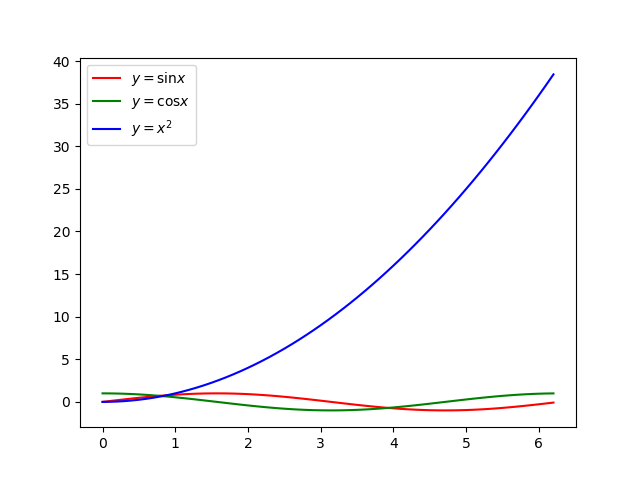
\includegraphics[width=\linewidth]{fig/func_vis.png}
	\caption{func\_vis.png}
	\label{fig1}
\end{figure}

\section{作业二}

\subsection{作业要求}

要求不用for循环实现双线性插值算法。

\subsection{具体实现}

代码如下,将图片缩小了两倍:

\begin{lstlisting}[title={inter\_linear.py}]
from PIL import Image

path=r'func_vis.png'
img=Image.open(path)
shape=img.size
img=img.resize((shape[0]//2,shape[1]//2), Image.BILINEAR)
img.save('fuc_vis_bilinear.png')
\end{lstlisting}

\subsection{运行结果}

如图\ref{fig2}所示。

\begin{figure}[htbp]
	\centering
	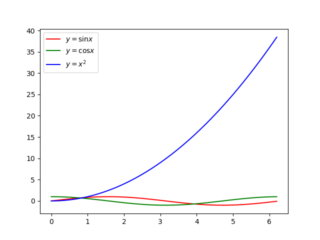
\includegraphics[width=0.5\linewidth]{fig/fuc_vis_bilinear.png}
	\caption{fuc\_vis\_bilinear.png}
	\label{fig2}
\end{figure}

%\end{CJK*}
\end{document}

